% !TeX spellcheck = en_US
\documentclass[10pt]{beamer}
\usepackage[utf8]{inputenc}
\usepackage[T1]{fontenc}
\usepackage{lmodern}
\usepackage[english]{babel}
\usetheme{CambridgeUS}
\usepackage{hyperref}
\hypersetup{
colorlinks=true,
linkcolor=blue,    
urlcolor=blue,
citecolor=blue,
}
\urlstyle{same}
\usepackage{graphicx}
\usepackage[backend=bibtex,style=authoryear]{biblatex}
\usepackage{enumerate}
\usepackage{siunitx}
\usepackage{subfig}
\usepackage{booktabs}
\addbibresource{references.bib} % Aggiungi il tuo file .bib

\DeclareSIUnit{\torr}{Torr}
\DeclareSIUnit{\at}{atoms}
\begin{document}




\title[CF-SMPCs]{Predicting Long-Term
Properties of Carbon Fiber-Reinforced Shape Memory Polymer
Composites in a Low Earth Orbit Environment. {\tiny (\cite{polym13101628})}}


\author[Andrea Marchegiani]{Andrea Marchegiani \\
\href{mailto:andrea.marchegiani@studenti.unitus.it}{ andrea.marchegiani@studenti.unitus.it}}




\institute[PCM]{ \\Master's Degree in Mechanical Engineering\\Polymer and Composites for Manufacturing}

\titlegraphic{\includegraphics[width=0.4\linewidth]{figures/Unitus_marchio_pdf}}


\date{16 September 2024}
%\setbeamercovered{transparent}
%\setbeamertemplate{navigation symbols}{}
\begin{frame}[plain]
\maketitle
\end{frame}



\begin{frame}
\frametitle{Table of contents}
\begin{enumerate}
\item \hyperlink{memory}{Shape-memory polymers}
\item \hyperlink{LEO}{Low earth orbit (LEO) environment}
\item \hyperlink{aim}{Aim of the research}
\item \hyperlink{introduction}{Introduction}			
\item \hyperlink{mm}{Materials and Methods}
\item \hyperlink{results}{Results}
\item \hyperlink{conclusions}{Conclusions}
\end{enumerate}
\end{frame}

\begin{frame}[label=memory]
\frametitle{Shape-memory polymers {\tiny \cite{BEHL200720}}}

\begin{columns}
\begin{column}{0.5\textwidth}
Shape-memory polymers are an emerging class of active polymers that
have dual-shape capability. \newline

They can actively change from a temporary shape A to a permanent shape B. \newline

Such applications can be found in: 
\begin{itemize}
\item Smart fabrics;
\item Heat shrinkable tubes;
\item Films for packaging;
\item Self deployable sun sails;
\item Implants for surgery;
\end{itemize}
\end{column}

\begin{column}{0.5\textwidth}
\begin{figure}[H]
\centering
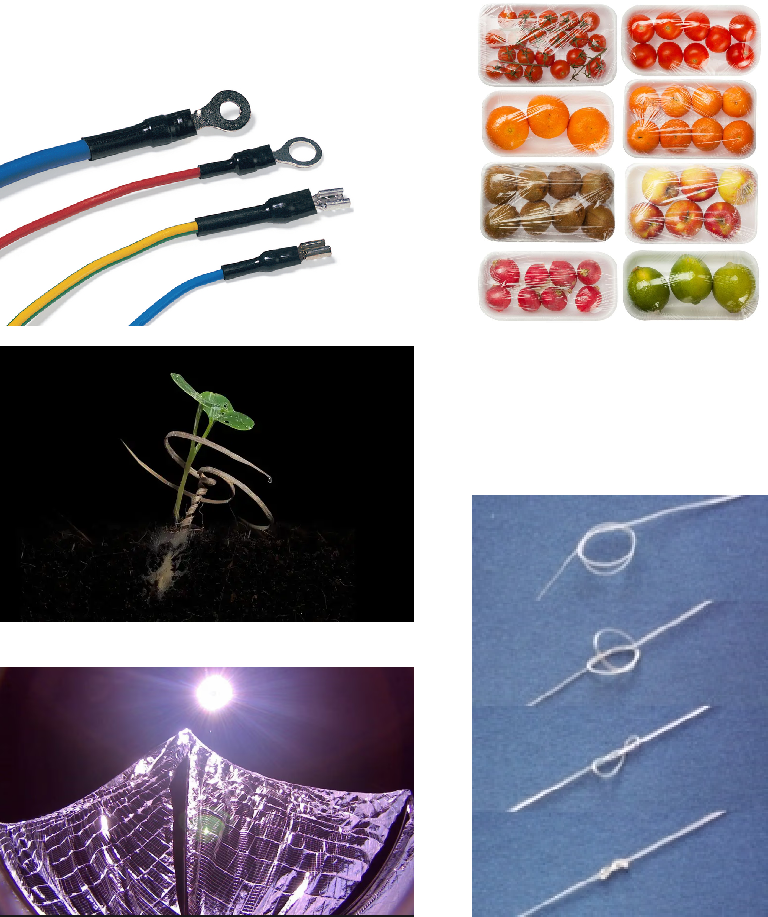
\includegraphics[width=0.85\linewidth]{tikz/imag_shape1}
\caption{Application of SMPs}
\label{fig:imagshape1}
\end{figure}     
\end{column}		
\end{columns}
\end{frame}


\begin{frame}
\small
The shape-memory effect in shape-memory polymers (SMPs) is not an inherent property but rather a result of their morphology and processing. Initially, the polymer is shaped into its permanent form B. In a process called \textbf{programming}, it is temporarily deformed into shape A. When an external stimulus is applied, the polymer reverts back to its permanent shape B.

The polymer network in an SMP consists of molecular switches and netpoints. These netpoints, which can be chemical (bond) or physical (intermolecular interactions), determine the permanent shape. Physical cross-linking occurs in block copolymers, where the domains with the highest thermal transition temperature $T_{perm}$ act as netpoints, while those with the second highest $T_{trans}$ act as molecular switches.
\begin{figure}[H]
\centering
\includegraphics[width=0.5\linewidth]{figures/screenshot001}
\caption{Molecular mechanism}
\label{fig:screenshot001}
\end{figure}	
				
\end{frame}

\begin{frame}

Shape-memory properties are quantified in cyclic ($N$) mechanical tests for the different stimuli. \newline

In these cyclic tests are tested:		
\begin{itemize}
\item  The \textbf{strain fixity rate} $R_f$, that quantifies the ability to fix a mechanical deformation $\varepsilon_m$, resulting in a temporary shape $\varepsilon_u(N)$;
\[R_f(N) = \dfrac{\varepsilon_u(N)}{\varepsilon_m}\]
\item  The \textbf{strain recovery rate} $R_r$, that quantifies the ability to restore the mechanical deformation of the permanent shape $\varepsilon_p(N)$ after application of a certain deformation $\varepsilon_m$;
\[R_r(N) = \dfrac{\varepsilon_m-\varepsilon_p(N)}{\varepsilon_m-\varepsilon_p(N-1)}\]

\item $T_{switch}$, switching temperature in case of thermal stimulation;
\end{itemize}			
\end{frame}

\begin{frame}
\footnotesize 
A typical stress-controlled programming cycle, follows four mainly steps. 

\begin{columns}
\begin{column}{0.5\textwidth}
\begin{figure}[H]
\centering
\includegraphics[width=0.8\linewidth]{figures/screenshot002}
\caption{Typical stress-strain-temperature diagram}
\label{fig:screenshot002}
\end{figure}
\end{column}
\begin{column}{0.5\textwidth}
\begin{enumerate}
\item $T>T_{trans}$ 

The sample is elongated to $\varepsilon_m$ while the molecular switches are open.

This strain is maintained for some time to allow relaxation of the polymer chains.


\item $T<T_{trans}$

The molecular switchers are closing while under the action of a constant stress $\sigma_m$

\item $T<T_{trans}$ 

The strain is reduced until a stress-free condition is
achieved at \SI{0}{\mega\pascal}.

\item $T>T_{trans}$

While the tensile stress is held constant at \SI{0}{\mega\pascal}, the molecular switches are opened
again, resulting in
the contraction of the test specimen and resumption of its permanent
shape.
\end{enumerate}
\end{column}
\end{columns}				
\end{frame}		


\begin{frame}[label=LEO]
\frametitle{Low earth orbit (LEO) environment}
Low Earth Orbit (LEO) is a popular location for satellite launches, but it presents several challenges for spacecraft due to its harsh environment. This environment includes atomic oxygen, ultraviolet radiation, ionizing radiation, ultra-high vacuum, thermal cycles, micrometeoroids, and orbital debris, all of which can degrade materials and electronic components. 

\begin{columns}
\begin{column}{0.5\textwidth}
\begin{itemize}
\item Variable altitudes:  200-1000\,\si{\kilo\meter}
\item Ultra-high Vacuum: \SI{5d-5}{\torr}
\item Thermal cycling: $\pm\SI{150}{\degreeCelsius}$
\item UV radiation: 100 - 200\,\si{\nano\meter}
\item Atomic Oxygen (AO) flux: \num{e13} - \num{e15}\,\si[per-mode = fraction]{\at\per\centi\meter\squared\per\second}
\item Orbital Debris at velocities of \SI[per-mode = fraction]{15}{\kilo\meter\per\second}
\item Satellite velocity \SI[per-mode = fraction]{8}{\kilo\meter\per\second}
\end{itemize}
\end{column}
\begin{column}{0.5\textwidth}
\begin{figure}[H]
\centering
\includegraphics[width=0.9\linewidth]{figures/LEO}
\caption{Orbital altitudes {\tiny Courtesy of Mark Mercer}}
\label{fig:leo}
\end{figure}
\end{column}
\end{columns}				
\end{frame}


\begin{frame}[label=aim]
\frametitle{Aim of the research}
\small

Carbon fiber-reinforced shape memory polymer composites (CF-SMPCs) have been researched
as a potential next-generation material for aerospace application, due to their lightweight
and self-deployable properties. 
\begin{figure}[H]
\centering
\includegraphics[width=0.9\linewidth]{tikz/imag_SMPC1}
\caption{Aerospace  application of SMPCs}
\label{fig:imagsmpc1}
\end{figure}
In this study was investigated the storage 
modulus ($G$) under simulation of a low Earth orbit (LEO) environment
involving three harsh conditions: high vacuum, atomic oxygen flux (AO) and ultraviolet (UV) light exposure. \newline

The effects of the three harsh
conditions on the properties of CF-SMPCs were characterized individually, using accelerated tests
conducted at various temperatures in a space environment chamber, and then, combined using
the time–temperature superposition principle (TTSP).

\end{frame}

\begin{frame}[label=introduction]
\frametitle{Introduction}

In the LEO environment:
\begin{itemize}
\item  High vacuum can lead to outgassing of polymer matrix
\item UV radiation can break the molecular bonds of the polymer
\item AO flux causes the surface erosion degrading the mechanical properties 
\item The temperature range can lead to microcracks due to the difference in the thermal expansion coefficient of the fiber and the matrix 
\end{itemize} 

So, accelerated test are commonly used to predict long-term properties and durability.
In short-duration experiments, accelerated tests are conducted under conditions that
are harsher than those of the target environment to project long-term performance. 

The TTSP provides the means to measure long-term behavior at a specific
temperature, by carrying out experiments at a higher temperature and within a shorter time. \newline 



\end{frame}

\begin{frame}[label=mm]
\frametitle{Materials and Methods}
\begin{columns}
\begin{column}{0.5\textwidth}
\textbf{Sample preparation}\\
\begin{itemize}
\item \textbf{Thermosetting continuous phase}\\
Epofix (Bisphenol A, BPA) + Jeffamine D-230 as diamine curing agent. 

\item \textbf{Fiber reinforced phase}\\
Four layers of TI-3101 woven carbon fabric.

\item \textbf{Manufacturing process}\\
Vacuum-assisted resin transfer molding.
\begin{itemize}
\item First curing at \SI{110}{\degreeCelsius} for \SI{3}{\hour}
\item Second curing at \SI{80}{\degreeCelsius} for \SI{2}{\hour}
\end{itemize}
\end{itemize}   
\end{column}

\begin{column}{0.5\textwidth}
\textbf{Environmental Chamber}\\

\begin{itemize}
\item High vacuum pump 
\item Cryogenic pump	
\item Deuterium lamps	
\item Plasma source with an ion accelerator 
\end{itemize}
\begin{figure}[H]
\centering
\includegraphics[width=0.9\linewidth]{figures/screenshot003}
\caption{Space environmental chamber}
\label{fig:screenshot003}
\end{figure}
\end{column}
\end{columns}
\end{frame}


\begin{frame}
\textbf{Characterization}\\
The storage modulus $G$ and glass
transition temperature $T_g$ were measured using:
\begin{itemize}
\item Three-point bending machine  
\item Termogravimetric analysis  
\item Fourier transform infrared spectra  
\item Field-emission scanning electron microscopy
\end{itemize}

\end{frame}

\begin{frame}[label=results]
\small
\frametitle{Results}
\textbf{Effects of AO Irradiation and Temperature on Matrix Erosion}\\
Surface morphology of AO-irradiated CF-SMPCs was observed, and erosion of the SMP matrix was confirmed
\begin{figure}[H]
\centering
\includegraphics[width=0.45\linewidth]{figures/screenshot005}
\caption{Effects of atomic oxygen (AO) exposure}
\label{fig:screenshot005}
\end{figure}
In general, the interface between the fiber and matrix is weakened due to the
effect of matrix erosion in an AO environment, resulting in degradation of the composite’s
mechanical properties. 
\end{frame}

\begin{frame}
\small
As the exposure temperature increased, Tg increased, whereas the $E$
decreased.  

% Please add the following required packages to your document preamble:
% \usepackage{booktabs}
\begin{table}[H]
\centering
\begin{tabular}{@{}ccc@{}}
\toprule
\textbf{AO Exposure} & \textbf{\begin{tabular}[c]{@{}c@{}}$T_g$\\ (\si{\degreeCelsius})\end{tabular}} & \textbf{\begin{tabular}[c]{@{}c@{}}TGA Onset\\ Temperature (\si{\degreeCelsius})\end{tabular}} \\ \midrule
Unexposed            & 70                                                                           & 344.98                                                                                       \\
70/21 \si{\hour}      & 71                                                                           & 349.82                                                                                       \\
110/21 \si{\hour}    & 73.5                                                                         & 349.17                                                                                       \\
150/21 \si{\hour}    & 84                                                                           & 361.67                                                                                       \\ \bottomrule
\end{tabular}
\end{table}
The erosion of the matrix by atomic oxygen (AO) can increase the weight fraction of the reinforcing material, leading to a higher glass transition temperature (Tg). However, the interaction between the polymer chains and the fibers can influence the chain kinetics in the area surrounding the fibers.
\begin{figure}[H]
\centering
\includegraphics[width=0.7\linewidth]{figures/screenshot007}
\label{fig:screenshot007}
\end{figure}

\end{frame}


\begin{frame}
FTIR spectroscopy let us notice three characteristic peaks:
\begin{enumerate}
\item  \SI{1250}{\per\centi\meter}  is related to the Ethylene oxide 
\item \SI{1509}{\per\centi\meter} is associated with N-H bond
\item \SI{1610}{\per\centi\meter} corresponds to the C-N bond
\end{enumerate}
\begin{figure}[H]
\centering
\includegraphics[width=0.7\linewidth]{figures/screenshot008}
\label{fig:screenshot008}
\end{figure}
TGA curves permit us to notice the temperature of degradation. 

The onset temperature before was smaller than the one obtained after AO flux at \SI{150}{\degreeCelsius}, this suggest the possibility of post-curing by AO: high energy breaks
the molecular chains inside the polymer, and the radicals generated create crosslinks. 
\end{frame}

\begin{frame}
\textbf{Quantitative Analysis of the AO Effect on Long-Term Properties}\\

Given that the AO effect accelerates with increasing exposure temperature, the TTSP was applied to evaluate the long-term properties due to this effect. \newline

Using the Arrhenius equation (eq. \ref{eq:1}, \ref{eq:2}), shifting values were calculated. Subsequently, a validation test was conducted using a new set of temperatures: 150 °C/21 h, 139 °C/50 h, 129 °C/100 h, 124 °C/150 h, and 120 °C/200 h, with different fiber orientations. \newline 

The results obtained were highly valid, demonstrating that the prediction model based on the acceleration test can be applied to polymer composites regardless of fiber orientation, as there were no significant differences among the five validation sets.

\end{frame}

\begin{frame}
\textbf{Acceleration Effects and Long-Term Properties under LEO Environment}\\
To obtain more accurate and representative results for the LEO environment, we will conduct accelerated tests that combine AO exposure with UV irradiation.\newline 

A significant trend observed is that, while applying harsher conditions increases $T_g$ as expected, the storage modulus now shows an upward trend, contrary to the behavior observed with AO flux alone.

This was because both UV and AO exposure
resulted in the formation of radicals via the breaking of bonds in the polymer matrix,
thereby causing post-curing to occur competitively.\newline 

Both UV and AO promoted post-curing, which resulted in an increase in
the storage modulus.

\end{frame}

\begin{frame}
\begin{figure}[H]
\centering
\subfloat{%
  \includegraphics[width=0.7\linewidth]{figures/screenshot010}
  \label{fig:screenshot010}
}\hfill
\subfloat{%
  \includegraphics[width=0.45\linewidth]{figures/screenshot011}
  \label{fig:screenshot011}
}
\label{fig:main_figure}
\end{figure}
\end{frame}

\begin{frame}
In order to provide the right shifting coefficient now we have to set: 
\[\log a_{LEO} = \alpha\log a_{UV} + \beta\log a_{AO}\]
And the choose of the right Arrhenius equation (eq. \ref{eq:3}) we can obtain the master curve.  
\begin{figure}[H]
\centering
\includegraphics[width=0.5\linewidth]{figures/screenshot012}
\label{fig:screenshot012}
\end{figure}
After exposure, post-curing was dominant in the early part; however,
in the second half of the curve, time-relaxation aging and AO-induced degradation
were prominent.
\end{frame}

\begin{frame}
The master curve displays a sort of viscoelastic behavior with a distinct peak attributed to UV- and AO-induced oxidative post-curing. The enhancement in storage modulus at the peak correlates with increased crosslink density, whereas the subsequent decrease may be associated with post-curing saturation or degradation. \newline 

Different exposure regimes influence the kinetics of post-curing, highlighting the complex interplay between environmental factors and the material's reactivity.
\end{frame}

\begin{frame}
\textbf{Shape Memory Properties under LEO Environment}\\
There was no significant change in
shape memory performance before and after exposure to the AO and LEO environments.
The fixity and recovery ratios were about 89\% and 97\%, respectively, indicating good shape
memory behavior.

\begin{figure}[H]
\centering
\subfloat[]{%
  \includegraphics[width=0.45\linewidth]{figures/screenshot013}
  \label{fig:screenshot013}
}\hfill
\subfloat[]{%
  \includegraphics[width=0.45\linewidth]{figures/screenshot014}
  \label{fig:screenshot014}
}
\label{fig:main_figure2}
\end{figure}
\end{frame}


\begin{frame}
The shape memory performance of epoxy-based thermosetting SMPCs was determined
based on the net points of the crosslinking structure and the flexible switching
segments. In this epoxy-based material, the crosslink points act as a net point like an anchor, while the main chain of epoxy acts as a flexible switching segment. As such, the
number of crosslink  can determine the shape memory performance. \newline 

In AO and LEO spaces, post-curing of CF-SMPCs progressed and crosslinking increased;
however, there was no further change in shape memory performance, as crosslinking
had already occurred sufficiently. 
\end{frame}

\begin{frame}[label=conclusions]
\frametitle{Conclusions}
In order to understand the underlying mechanisms governing the degradation of CF-SMPCs in a LEO environment, it is imperative to delve into their performance characteristics:
\begin{enumerate}
\item \textbf{AO environment}\\
Surface erosion leading to smaller $G$ and higher $T_g$ due to the rise of weight fraction of the reinforcing material. 

\item \textbf{LEO environment}\\
Post curing process leading to higher $G$ and $T_g$ due to the formation of more cross-linked radicals.
\end{enumerate}
\end{frame}

\begin{frame}
\frametitle{Thank you for your attention}
\begin{figure}[H]
\centering
\includegraphics[width=\linewidth]{figures/immagine_finale}
\label{fig:immaginefinale}
\end{figure}

\end{frame}

\begin{frame}
\frametitle{References}
\printbibliography
\end{frame}



\begin{frame}
\frametitle{Appendix A - ASTM-E2089}
The AO flux in this environment was verified
based on the ASTM-E2089 standard, in which the AO flux is predicted based on the
mass change of a reference material: Kapton. 
\[f = \dfrac{\Delta M}{A\rho Et}\]
where $f$ is the effective AO flux, $\Delta M$ is the mass change of the reference materials, $A$ is the
exposed area, $\rho$ is the density, $E$ is the erosion yield, and $t$ is the exposure duration. The
AO flux was calculated based on the mass loss measured over a 21-h exposure period.
\end{frame}

\begin{frame}
\frametitle{Appendix B - TTSP Arrhenus formulations}

\begin{equation}\label{eq:1}
G(t,T^{AO}) = G^{ref}\left(\dfrac{t}{a_{AO}(T)}, T^{AO, ref}\right)
\end{equation}
where $G^{ref}$ refers to the storage modulus of CF-SMPCs exposed at the reference temperature,
$T^{AO, ref}$is the reference exposure temperature (70 \si{\degreeCelsius}), $a_{AO}(T)$ is the shift factor at
the exposure temperature, and $G$ is the predicted storage modulus of CF-SMPCs at the
exposure temperature.
\begin{equation}\label{eq:2}
\log a_{AO}(T) = \dfrac{\Delta H_{T, AO}}{2.303R}\left(\dfrac{1}{T^{AO}} - \dfrac{1}{T^{AO, ref}} \right)
\end{equation}
Where $\Delta H_{T, AO}$ is the activation energy that for the AO process was 84.16 KJ/mol.
\end{frame}

\begin{frame}
\begin{equation}\label{eq:3}
G(t,T,T^{LEO}) = G^{ref}\left(\dfrac{t}{a_T(T)a_{LEO}(T)}, T^{ref}, T^{LEO, ref}\right)
\end{equation}
\end{frame}
\end{document}